% Introduction to Newton's Method
% Source: https://stats.stackexchange.com/questions/376191/why-is-the-second-derivative-required-for-newtons-method-for-back-propagation
% Source: https://tutorial.math.lamar.edu/classes/calci/newtonsmethod.aspx
% Source: https://ardianumam.wordpress.com/2017/09/27/newtons-method-optimization-derivation-and-how-it-works/
% Spring 2021



\qns{Newton's Method Introduction}

\meta{In this problem, we will review Newton's method, which was introduced in lecture.}

The newton's method that you may have heard of in calculus class is typically used for finding the roots of a function.
Recall that the roots of a function are the inputs such that the output is zero.

Suppose that we have the function $f(x) = x^{2} + 5x + 6$.
Factorizing into $f(x) = (x+2)(x+3)$ reveals that the roots of this function are $x=-2, -3$.

\begin{center}
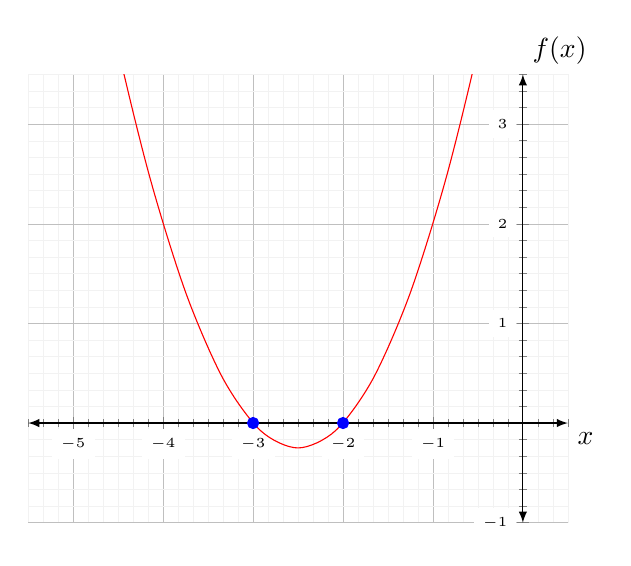
\begin{tikzpicture}
  \begin{axis}[
    xmin=-5,xmax=0,
    ymin=-0.5,ymax=3,
    grid=both,
    grid style={line width=.1pt, draw=gray!10},
    major grid style={line width=.2pt,draw=gray!50},
    axis lines=middle,
    minor tick num=5,
    enlargelimits={abs=0.5},
    axis line style={latex-latex},
    ticklabel style={font=\tiny,fill=white},
    xlabel style={at={(ticklabel* cs:1)},anchor=north west},
    ylabel style={at={(ticklabel* cs:1)},anchor=south west},
    xlabel=$x$,
    ylabel=$f(x)$
] 
    \addplot[smooth, red] {x^2 + 5*x +6}; 
    \addplot[only marks, blue]
        coordinates
        {(-3, 0) (-2, 0)};
  \end{axis}
\end{tikzpicture}
\end{center}

\begin{enumerate}

\qitem

However, suppose that we didn't know how to factorize and want an iterative algorithm to estimate these roots.
Let's say that we started off with a point $x_0=-1$ that just happens to be the right of $x=-2$. 
Calculate the tangent line at this point and draw it on the graph. 


\begin{center}
    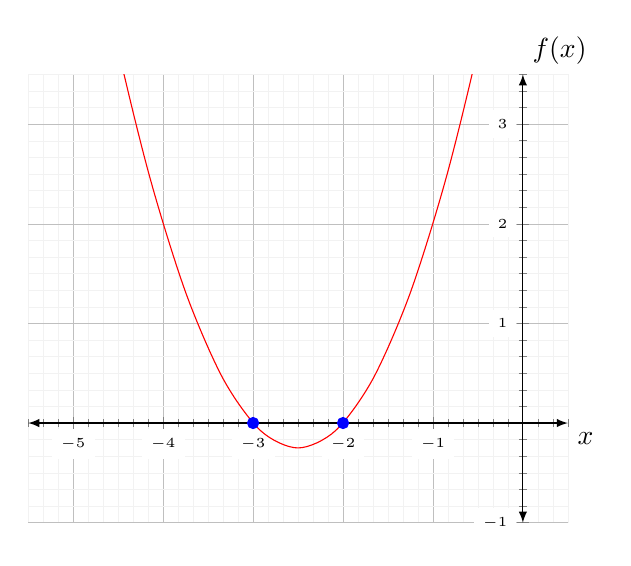
\begin{tikzpicture}
        \begin{axis}[
        xmin=-5,xmax=0,
        ymin=-0.5,ymax=3,
        grid=both,
        grid style={line width=.1pt, draw=gray!10},
        major grid style={line width=.2pt,draw=gray!50},
        axis lines=middle,
        minor tick num=5,
        enlargelimits={abs=0.5},
        axis line style={latex-latex},
        ticklabel style={font=\tiny,fill=white},
        xlabel style={at={(ticklabel* cs:1)},anchor=north west},
        ylabel style={at={(ticklabel* cs:1)},anchor=south west},
        xlabel=$x$,
        ylabel=$f(x)$
    ] 
        \addplot[smooth, red] {x^2 + 5*x +6}; 
        \addplot[only marks, blue]
            coordinates
            {(-3, 0) (-2, 0)};
        \end{axis}
    \end{tikzpicture}
    \end{center}

    \sol{
        Calculating derivative of $f(x)$ yields $f'(x) = 2x + 5$.
        Thus, $f'(-1) = 3$.
        We also know that $f(-1) = 2$. 
        Using the equation for a linear line, we get that the tangent line is 
        \begin{equation}
            y = 3x + 5
        \end{equation}
    }

    \qitem 
    Where does the tangent line cross the x axis? 

    \sol{
        Setting $0 = 3x + 5$, we have $x = -\frac{5}{3}$.
    }

    \qitem 
    Calculate the tangent line at the $x$ computed in the previous part and find the intersection between this new line and the x axis.
    
    \sol{
        The slope at $x = -\frac{5}{3}$ is \[ f'(-\frac{5}{3}) = \frac{5}{3}\]
        Also, \[f(-\frac{5}{3}) = \frac{4}{9}\]
        Therefore, the tangent line is 
        \begin{equation}
            y = \frac{5}{3}x + \frac{29}{9}
        \end{equation}
    }

    \qitem 
    Notice that as we keep doing this we'll eventually hit $x = -2$ and thus hit one of the roots of our function. 
    This process we're performing is the essence of newton's method:
    \begin{enumerate}
        \item Start off with a guess of the root of our function $f(x)$ that we'll call $x_0$.
        \item Calculate the tangent line at the point $x_0$ using $f'(x)$.
        \item Find the intersection of this tangent line with the x-axis.
        \item This intersection has an $x$ which we'll call $x_1$. 
        \item Repeat steps $ii$ through $iv$ with the new $x_i$ until we've hit a root.
    \end{enumerate}
    Using the previous parts and substituting variables where need be, write an equation that explains how our $x$'s are evolving.

    \sol{
        Initially, we start off with the following set of equations for $x_0$. 
        $x_0$ is an actual point, we use it as a subscript to denote the corresponding tangent line.
        
        \begin{align}
        y_{x_0} = m_{x_0} x_{x_0} + b_{x_0} \\
        f(x_0) = f'(x_0)x_{x_0} + b_{x_0} \\
        b = f(x_0) - f'(x_0)x_{x_0} \\
        f(x_{x_0}) = f(x_0) + f'(x_0) * (x_{x_0} - x_0)
        \end{align}
        
        Recall that we defined $x_1$ as the the point where the $x_0$ tangent line intersects with the x-axis.
        Thus, we can plug in $x_1$ and get the following:
        \begin{equation}
            0 = f(x_0) + f'(x_0) * (x_1 - x_0) 
        \end{equation}

        Rearranging, we get 
        \begin{equation}
            x_1 = x_0 - \frac{f(x_0)}{f'(x_0)}
        \end{equation}

        In a given iteration $i$, that means we have 
        \begin{equation}
            x_{i+1} = x_i - \frac{f(x_i)}{f'(x_i)}
        \end{equation}
    }

    At this point, it's important to note that this algorithm definitely has flaws.
    The most obvious one is that we need derivatives or else we get division by zero.
    Additionally, the initial $x_0$ that we choose will affect which roots we get. 
    You can imagine that depending on where these initial $x_0$ are, you might not get all the roots.
    There are also many other issues that won't be discussed here.

    \qitem 
    Notice that for our original formulation, we wanted to find the roots of a given function.
    How might we adapt this algorithm to find minimum or maximum of a given function?
    What would our evolution equation look like now?
    \emph{HINT: Use a second order taylor approximation and set it to zero.}

    \sol{
        We want to apply a similar philosophy as before, but this time we want to find the values of $x$ such that we get a derivative $f'(x) = 0$.
        Thus, starting off with $x_0$, we use the hint and take a second order taylor series approximation. 
        We get
        \begin{equation}
            f(x_{x_0}) \approx f(x_0) + f'(x_0)(x_{x_0} - x_0) + \frac{1}{2} f''(x_0)(x_{x_0} - x_0)^{2}
        \end{equation}
        We want to set the derivative to be 0, so we take the derivative of the approximation and set it to 0.
        This leads us to 
        \begin{equation}
            f'(x_0) \approx f'(x_0) + f''(x_0)x_{x_0} - f''(x_0)x_0 = 0
        \end{equation}
        Rearranging, we get
        \begin{equation}
            x_1 = x_{x_0} = \frac{f''(x_0)}{f''(x_0)}x_0 - \frac{f'(x_0)}{f''(x_0)}
        \end{equation}
        We set the found $x_{x_0} = x_1$ because this $x_1$ is the value of $x_{x_0}$ for which the tangent line of the derivative hits the x-axis.\
        To put it differently, we're doing the same thing as earlier, but using it on the first derivative $f'(x)$ rather than $f(x)$.
        Our new evolution equation is therefore 
        \begin{equation}
            x_{i+1} = x_{i} - \frac{f'(x_i)}{f''(x_{i})}
        \end{equation}
    }

    This second form of newton's method is the one that is very much used in machine learning because it can find local extremum.
    However, it suffers similar flaws as the first form of newton's method such as having to have a second order derivative be non zero, etc.
    The matrix vector version of this algorithm was what was covered in lecture 13B.


\end{enumerate}

